\chapter{Đề thi THPT Lịch sử}
\label{chap:appendix_exam}
\begin{figure}[htbp]
    \centering
    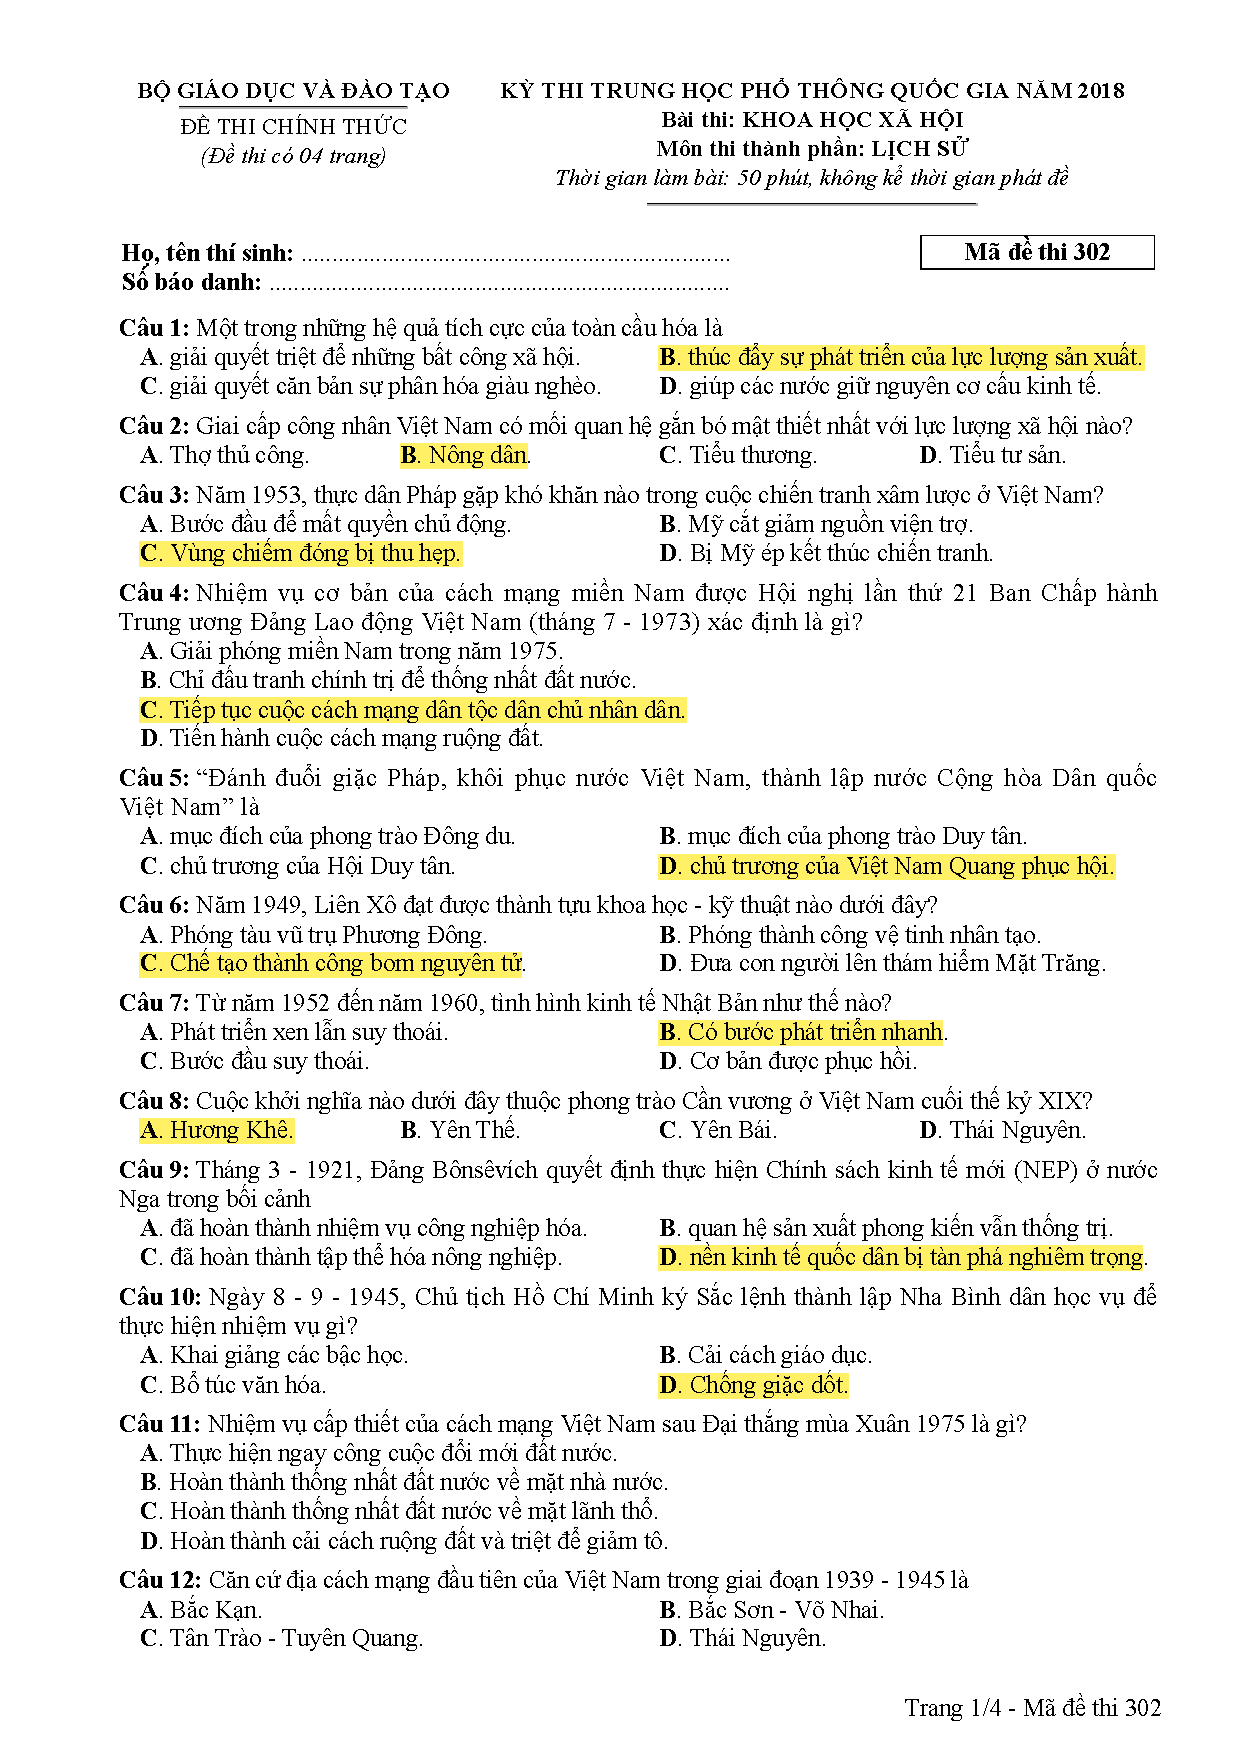
\includegraphics[width=1\textwidth, page=1]{Appendix/Fig/2018_302.pdf}
    \caption{Trang 1 đề thi THPT Lịch sử 2021}
\end{figure}

\begin{figure}[htbp]
    \centering
    \includegraphics[width=1\textwidth, page=2]{Appendix/Fig/2018_302.pdf}
    \caption{Trang 2 đề thi THPT Lịch sử 2021}
\end{figure}

\begin{figure}[htbp]
    \centering
    \includegraphics[width=1\textwidth, page=3]{Appendix/Fig/2018_302.pdf}
    \caption{Trang 3 đề thi THPT Lịch sử 2021}
\end{figure}

\begin{figure}[htbp]
    \centering
    \includegraphics[width=1\textwidth, page=4]{Appendix/Fig/2018_302.pdf}
    \caption{Trang 4 đề thi THPT Lịch sử 2021}
\end{figure}


\begin{table}[ht]
    \centering
    \caption{Câu trả lời của phương pháp đề xuất cho đề thi THPT Lịch sử 2018, mã đề 302. Với các câu in đậm là câu trả lời sai}
    \resizebox{\textwidth}{!}{
        \small
        \begin{tabular}{|>{\centering\arraybackslash}m{1.5cm}|*{10}{>{\centering\arraybackslash}m{1cm}|}}
            \hline
            \textbf{Câu}    & 1  & 2           & 3  & 4           & 5  & 6  & 7  & 8  & 9  & 10          \\ \hline
            \textbf{Đáp án} & B  & B           & C  & C           & D  & C  & B  & A  & D  & D           \\ \hline
            \textbf{Câu}    & 11 & 12          & 13 & 14          & 15 & 16 & 17 & 18 & 19 & 20          \\ \hline
            \textbf{Đáp án} & B  & B           & A  & C           & C  & C  & A  & B  & B  & B           \\ \hline
            \textbf{Câu}    & 21 & 22          & 23 & \textbf{24} & 25 & 26 & 27 & 28 & 29 & \textbf{30} \\ \hline
            \textbf{Đáp án} & A  & D           & D  & \textbf{D}  & B  & B  & A  & C  & A  & \textbf{C}  \\ \hline
            \textbf{Câu}    & 31 & \textbf{32} & 33 & 34          & 35 & 36 & 37 & 38 & 39 & 40          \\ \hline
            \textbf{Đáp án} & D  & \textbf{C}  & D  & A           & C  & A  & B  & C  & D  & C           \\ \hline
        \end{tabular}
    }
\end{table}
